\documentclass {beamer}	
\usepackage{amsmath}
\usepackage{amsfonts}
\usepackage{amssymb}
\usepackage{multimedia}
\usepackage[T2A]{fontenc}
\usepackage[utf8]{inputenc}
\usepackage[english,russian]{babel}
\usepackage{graphicx}
\usepackage{wrapfig}
\uselanguage{Russian}
\languagepath{Russian}
\deftranslation[to=Russian]{Theorem}{Теорема}
\deftranslation[to=Russian]{Definition}{Определение}

\usetheme{PaloAlto}
\usefonttheme{structureitalicserif}

\title{Динамические игры на временных шкалах}
\author {Выполнил: Бондаренко Алексей \\Научный руководитель: Плотников~А.~В., соруководитель Огуленко~А.~П.}
\date{}


\begin{document}

\begin{frame}
\maketitle
\end{frame}

\begin{frame}
\section{Постановка задания}
\frametitle{Постановка задания}
\begin{itemize}
	\item Изучить модель инфляционной политики Либиха и Штекеля. 
	\item Изучить классическую модель конфликта профсоюз---монополист.
	\item Построить динамическую игру на временных шкалах для модели профсоюз---монополист.
	\item Путем имитационного моделирования изучить свойства макроэкономических моделей.
\end{itemize}
\end{frame}

\begin{frame}
\section{Модель Либиха"--~Штекеля}
\frametitle{Модель Либиха"--~Штекеля}
В игре участвуют два игрока: 
\begin{enumerate}
	\item $g$ --- правительство, оперирующее декларируемым уровнем инфляции $\pi$
	\item $p$ --- общественность, требующая индексации зароботной платы на уровне $\omega$
\end{enumerate}

Каждый игрок может установить управляемый им параметр либо на низком, либо на высоком уровне.

\end{frame}

\begin{frame}
\frametitle{Модель Либиха"--~Штекеля. Биматричная игра}
В общем виде игра может быть задана в виде матрицы выигрышей
\begin{figure}[h!]
	\centering
	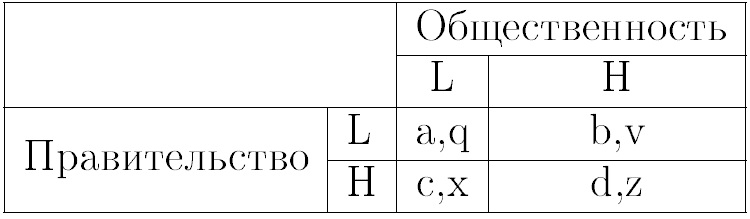
\includegraphics[width=0.5\textwidth]{first}
\end{figure}

где выигрыши удовлетворяют ограничениям

\begin{gather}	
\label{eq:sec:ot:constraint}
	c > a = 0 > d > b, \qquad c = -d = -\frac{b}{2}, \\
	q > v, \qquad q \geqslant z > x
\end{gather}

Эти соотношения вытекают из макроэкономической модели Барро"--~Гордона,
основанной на теории полезности.
\end{frame}

%\begin{frame}
%\frametitle{Идея решения}
%Экономику зададим через функцию совокупного предложения Лукаса
%$$y_t - Y = \lambda(\pi_t - \omega_t)+\varepsilon_t,$$
%где  $\lambda>0, y$  – производительность, $Y$ – естественный уровень производительности, а  $\varepsilon$ - макроэкономический шок близкий к нулю.
%Функции полезности: 
%$$ u^g_t=-(\pi_t - \tilde{\pi})^2 + \alpha y_t - \beta(y_t-Y)^2,$$
%$$ u^p_t=-(\pi_t - \omega)^2,$$
%
%где $\tilde{\pi}$ - оптимальный уровень инфляции, а $\alpha > 0, \beta > 0$ описывают относительный вес целей правительствa.
%\end{frame}


%\begin{frame}
%\frametitle{Идея решения}
%Было получено равновесие 
%$$ \pi^*_t= \tilde{\pi} + \frac{\alpha\lambda}{2}= \omega^*_t,$$ 
%Ли и Чао предлагают два наиболее оптимальных варианта 
%$$\pi \in \left\{L=\tilde{\pi}, H=\tilde{\pi}+\frac{\alpha\lambda}{2} \right\} \ni $$
%В связи с чем были выведены следующие соотношения между выигрышами:
%\begin{equation}
%\label{eq:sec:ot:constraint}
%c>a=0 > d > b,c=-d=-\frac{b}{2}, q>v,q\ge z>x
%\end{equation}
%\end{frame}

%\begin{frame}
%\frametitle{Идея решения}
%Положим в соответствии с имеющимися ограничениями
%$$c=1 > a=0 > d=-1 > b=-2, q=z=0 > v=x=-1,$$
%  \begin{center}
%  	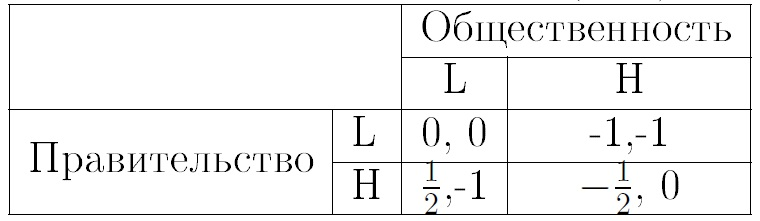
\includegraphics[width=0.5\textwidth]{second}
%  \end{center}
%  
%  Стандартная пошаговая игра имеет уникальное равновесие по Нэшу $(H,H)$. Однако, оно неэффективно, так как является Парето доминированным.
%  Парето-оптимальным будет  $(L,L)$
%\end{frame}


\begin{frame}
\frametitle{Модель Либиха"--~Штекеля. Асинхронная игра}
\begin{enumerate}
	\item Игра начинается одновременным ходом
	\item Заранее известно неизменное количество ходов правительства $r^g
		\in \mathbb{N}$ и общественности $r^p \in \mathbb{N}$
	\item Игра заканчивается через $T$ тактов времени, где $T$ --- НОК($r^g$,$r^p$)
	\item Игроки рациональны, обладают равноценными знаниями и полной
		информацией о структуре игры, матрице выигрышей и всех
		предыдущих ходах
\end{enumerate}
\end{frame}

\begin{frame}
\frametitle{Модель Либиха"--~Штекеля. Асинхронная игра}
Определяется три временных шкалы: правительства, общественности и общая шкала игры:
\begin{gather}
	\label{eq:sec:tech:scales}
	T_g = \{0,r^g,2r^g,...,T\}, \qquad T_p=\{0,r^p,2r^p,...,T\}, \\
	T = T_g \cup T_p 	
\end{gather}
	
Асинхронная игра на временных шкалах будет, вообще говоря, иметь несколько
равновесий по Нэшу, среди которых логично выбрать наилучшее по всем подыграм.
\begin{definition}
	Любое совершенное равновесие по подыграм (SPNE), в котором оба игрока
	выбирают Парето-оптимальную стратегию  во всех своих ходах, назовём
	\textbf{совершенным равновесием Рамсея по подыграм (Ramsey SPNE)}
\end{definition}
\end{frame}


\begin{frame}
\frametitle{Модель Либиха"--~Штекеля. Устойчивость}
	\begin{theorem}
	\small	Рассмотрим асинхронную игру на временных шкалах (3), (4), 
	для которой выполняются условия (1) и (2). Тогда все SPNE игры будут SPNE типа Рамсея,
	если и только если 
	{\scriptsize
		\begin{equation}
		\label{eq:sec:tech:theoremSystem}
		r^g> \bar{r^g}(R) = \left\{ 
		\begin{aligned} 
		&\frac{c - d}{a-d}r^p= \frac{a-b}{a-d}r^p, &&\text{если } R=0
		\\
		&\frac{(1+R)(c-d)}{a-d}r^p= \frac{a-b + R(c-d)}{a-d}r^p, &&\text{если } 	R\in(0; \bar{R})
		\\
		&\frac{c-d-(1-R)(a-b)}{a-d}r^p= \frac{(a-b)}{a-d}Rr^p, &&\text{если } 	R\in(\bar{R};1)
		\end{aligned}
		\right.		
		\end{equation}
	}
	где $\bar{R}=\frac{q-v}{z-x+q-v}$. 
\end{theorem}

Теорема устанавливает связь между устойчивостью стратегий и <<подвижностью>>
игроков.
\end{frame}

\begin{frame}
\frametitle{Модель Либиха"--~Штекеля. Имитация игры}
	Для компьютерного моделирования взята модель с матрицей выигрыша
	  \begin{center}
	  	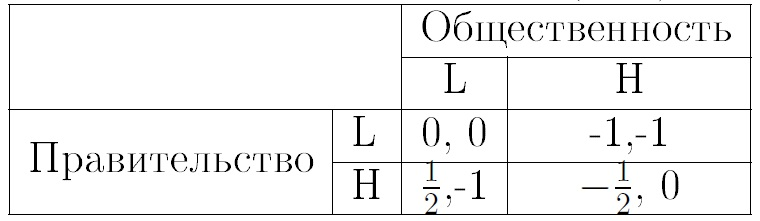
\includegraphics[width=0.5\textwidth]{second}
	  \end{center}
	и количеством ходов игроков $r^g= 7$ и $r^p= 4$.
	
	Рассмотрим случай, когда правительство скорее склонно ввести высокий
	уровень инфляции, а общественность предполагая, что правительство
	пойдет на этот шаг, с высокой долей вероятности потребует повышения зарплат.	
\end{frame}

\begin{frame}
\frametitle{Модель Либиха"--~Штекеля. Имитация игры}
	
	 \begin{gather*}
	 q^g = \left[ 0.5; 0.9; 0.7; 0.5; 0.9; 0.73; 0.8 \right], \\
	 q^p = \left[ 0.8; 0.9; 0.8; 1 \right].
	 \end{gather*}
	 \begin{figure}
	 	\begin{minipage}[b]{0.45\textwidth}
	 		
	 	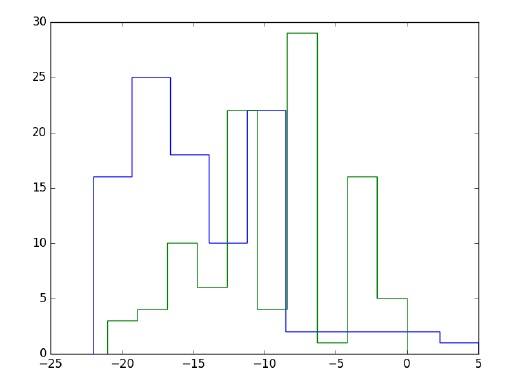
\includegraphics[width=\textwidth]{government1}
	 \end{minipage}
	 \begin{minipage}[b]{0.45\textwidth}
	 	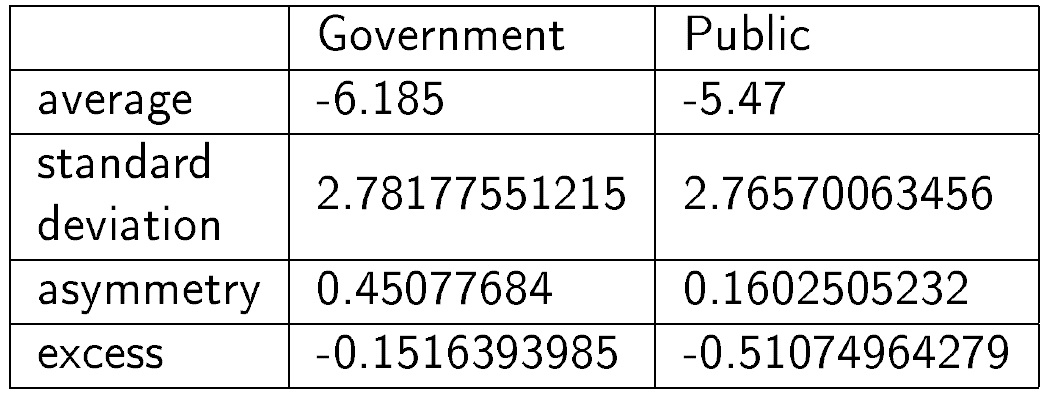
\includegraphics[width=\textwidth]{third}
	 \end{minipage}
	 
	 \end{figure}


%Согласно полученным результам легко видеть, что подобный набор стратегий невыгоден обеим сторонам, к тому же правительству из-за более "мягкого" подхода "более невыгодно".
\end{frame}

\begin{frame}
\frametitle{Модель Либиха"--~Штекеля. Имитация игры}
 \begin{gather*}
 q^g = \left[ 0; 0; 0; 0; 0; 0; 0.3 \right], \\
 q^p = \left[ 0; 0; 0; 0 \right].
 \end{gather*}
 
\begin{figure}
	\begin{minipage}[b]{0.45\textwidth}
		
		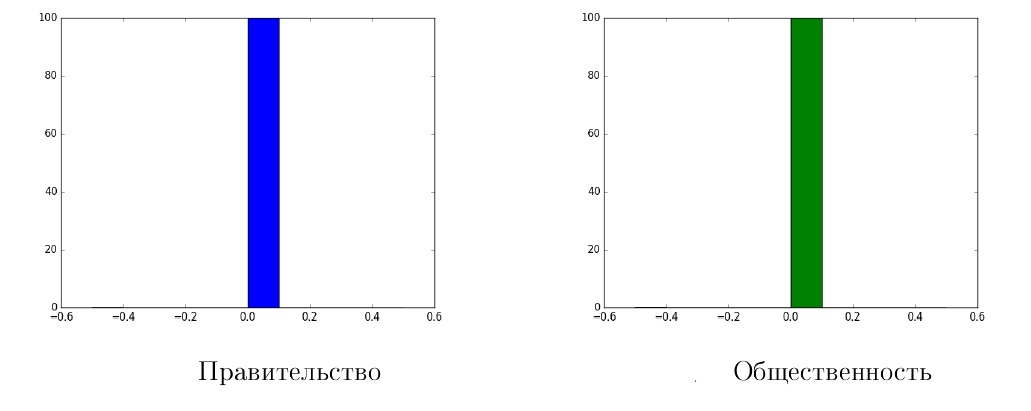
\includegraphics[width=\textwidth]{forth}
	\end{minipage}
	\begin{minipage}[b]{0.45\textwidth}
		
		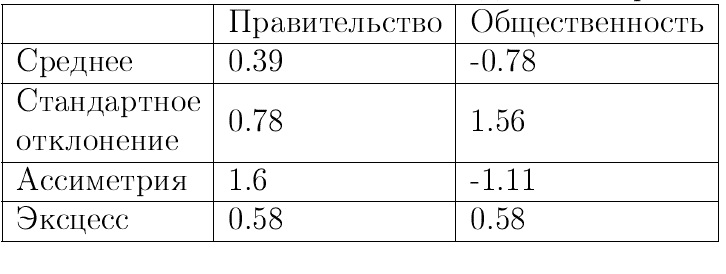
\includegraphics[width=\textwidth]{fifth}
	\end{minipage}
	
\end{figure}
	
%Данная стратегия является Парето-оптимальной, игрокам нет смысла отклоняться от неё в долгосрочной перспективе.
\end{frame}


\begin{frame}
\frametitle{Модель Либиха"--~Штекеля. Имитация игры}
 \begin{gather*}
 q^g = \left[ 0; 0; 0; 0; 0; 0; 0.3 \right], \\
 q^p = \left[ 0; 0; 0; 0.15 \right].
 \end{gather*}
	
	\begin{figure}
		\begin{minipage}[b]{0.45\textwidth}
			
			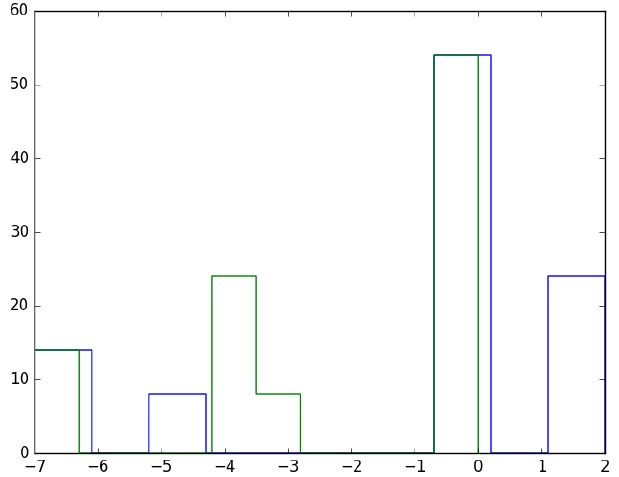
\includegraphics[width=\textwidth]{10th}
		\end{minipage}
		\begin{minipage}[b]{0.45\textwidth}
			
			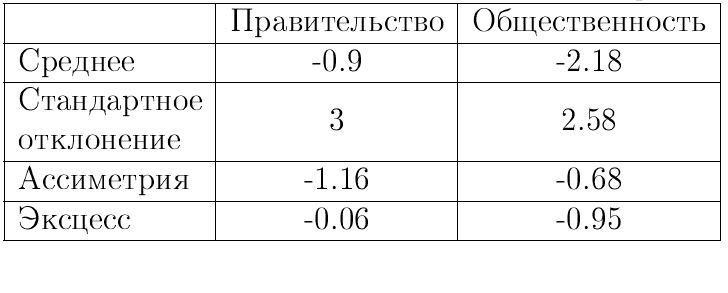
\includegraphics[width=\textwidth]{11th}
		\end{minipage}
		
	\end{figure}
	
	%Данная стратегия является Парето-оптимальной, игрокам нет смысла отклоняться от неё в долгосрочной перспективе.
\end{frame}

\begin{frame}
\frametitle{Модель Либиха"--~Штекеля. Имитация игры}
 \begin{gather*}
 q^g = \left[ 0; 0; 0; 0; 0; 0; 0.3 \right], \\
 q^p = \left[ 0; 0; 0; 0.8 \right].
 \end{gather*}
	\begin{figure}
		\begin{minipage}[b]{0.45\textwidth}
			
			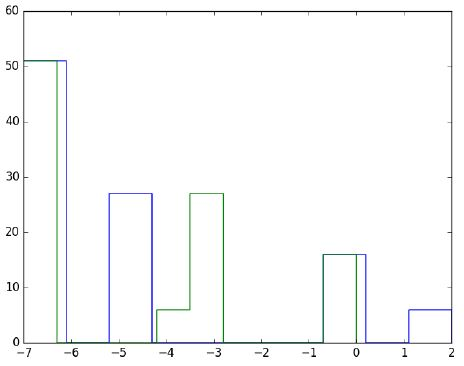
\includegraphics[width=\textwidth]{12th}
		\end{minipage}
		\begin{minipage}[b]{0.45\textwidth}
			
			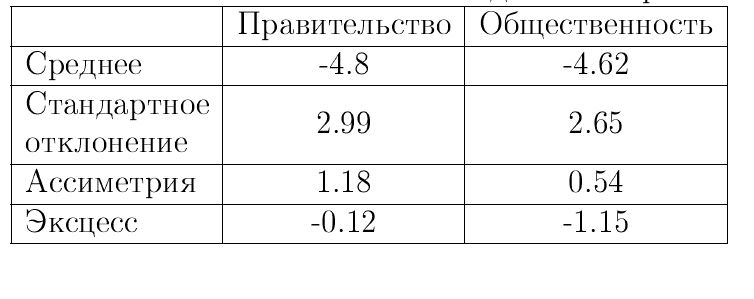
\includegraphics[width=\textwidth]{13th}
		\end{minipage}
		
	\end{figure}
	
	%Данная стратегия является Парето-оптимальной, игрокам нет смысла отклоняться от неё в долгосрочной перспективе.
\end{frame}


\begin{frame}
\section{Модель профсоюз---монополист}
\frametitle{Конфликт профсоюз---монополист}
Данная модель является моделью отношений между профсоюзом и фирмой--монополистом, 
в которой профсоюз задаёт уровень заработной платы $W$, а фирма определяет 
количество наёмных работников $E$ (уровень найма).

\end{frame}

\begin{frame}
\frametitle{Конфликт профсоюз---монополист}
Функция полезности профсоюза имеет вид 
$$ U = U(W,E), \quad \frac{\partial U}{\partial W} > 0; \quad \frac{\partial U}{\partial E}~>~0.$$ 
Например $U = \lambda WE$, где $\lambda \in (0; 1)$\\
Полезность для фирмы измеряется как прибыль 
$$\Pi~=~PY(\bar K,E)~-~WE,$$ 
где цена $P$ дана, а капитал $\bar K$ фиксирован. Отсюда мы можем переписать 
$$\Pi(W,E)~=~R(E)~-~WE,$$ 
где $R$ -- доход.
\end{frame}

\begin{frame}
\frametitle{Конфликт профсоюз---монополист. Классическое решение}
	
	Фирма максимизирует свою прибыль по $E$ при заданном уровне заработной платы. 
	Необходимое условие оптимальности примет вид
	$$ W = R'(E).$$
	Разрешая уравнение относительно $E$, получим кривую спроса: $$E~=~g(W)$$\\
	Профсоюз со своей стороны решает задачу
	$$ \max_W U(W,E) = U(W,g(W)). $$
\end{frame}


\begin{frame}
\frametitle{Конфликт профсоюз---монополист. Классическое решение}

 \begin{center}
 	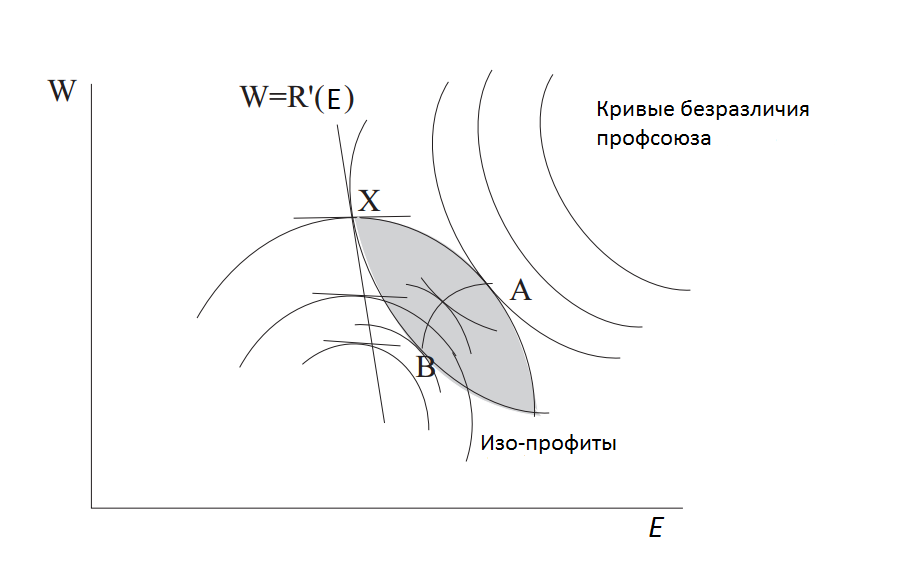
\includegraphics[width=0.8\textwidth]{monopoly_union}
 \end{center}
 Точка $X$ --- точка равновесия.  $AB$ --- кривая контракта, состоящая из
 точек, в которых изопрофиты и кривые безразличия профсоюза имеют общую касательную.
\end{frame}

\begin{frame}
	
\frametitle{Конфликт профсоюз---монополист. Биматричная игра}
	
\begin{itemize}
	\item Профсоюз устанавливает уровень зарплаты $W$
	\item Фирма задает количество нанимаемых рабочих $E$
\end{itemize}

Каждый игрок выбирает между низким и высоким уровнем параметра.
	\begin{center}
		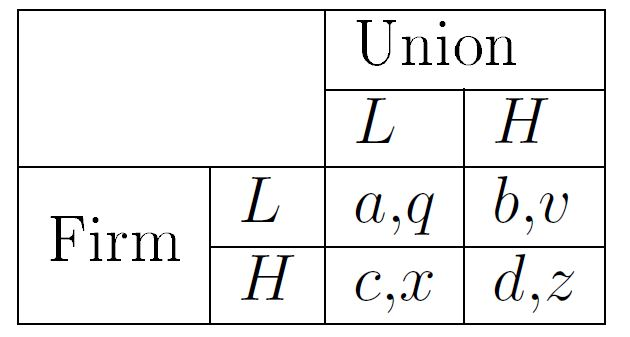
\includegraphics[width=0.5\textwidth]{sixth}
	\end{center}
\end{frame}


\begin{frame}
	
\frametitle{Конфликт профсоюз---монополист. Биматричная игра}
	Функция полезности профсоюза  $U(W,E)=\lambda WE$, где $\lambda \in(0;1)$:
	$$
	\frac{\partial U}{\partial W} > 0; 
	\quad 
	\frac{\partial U}{\partial E}~>~0 ; 
	\quad
	\frac{\partial^2 U}{\partial W^2} \leqslant 0
	$$
	
	$$
	U(0,E) = U(W,0) = U(0,0) = 0.
	$$
	
	
	Функция полезности фирмы $\Pi(W,E)=cP(\bar{K},E)-WE$:
	$$P(\bar{K}, E)=A\bar{K}^\alpha E^\beta,$$  где $A$ – коэффициент нейтрального технического прогресса, $\alpha$ и $\beta$ – коэффициенты эластичности валового внутреннего продукта по капитальным и трудовым затратам.\\
\end{frame}

\begin{frame}
\frametitle{Конфликт профсоюз---монополист. Биматричная игра}
 \begin{center}
 	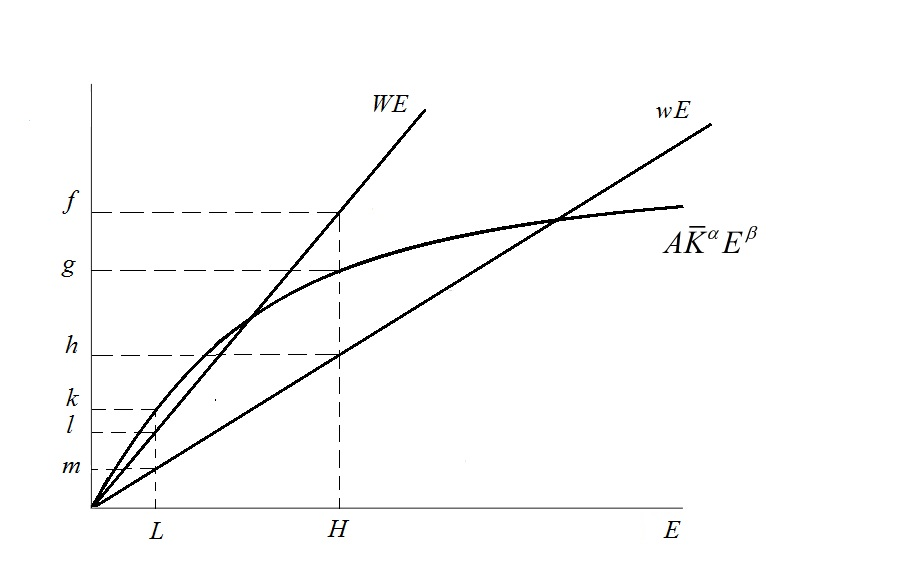
\includegraphics[width=0.8\textwidth]{monopoly_union2}
 \end{center}
		$$U(L,L) < U(L,H) \nsim U(H, L) < U(H,H)$$
		$$\Pi(H,H) < \Pi(H,L) < \Pi(L, L) < \Pi(L,H)
		 $$

\end{frame}

\begin{frame}
\frametitle{Конфликт профсоюз---монополист. Имитация}
		Пусть матрица выигрышей имеет следующий вид:
		
		\begin{center}
			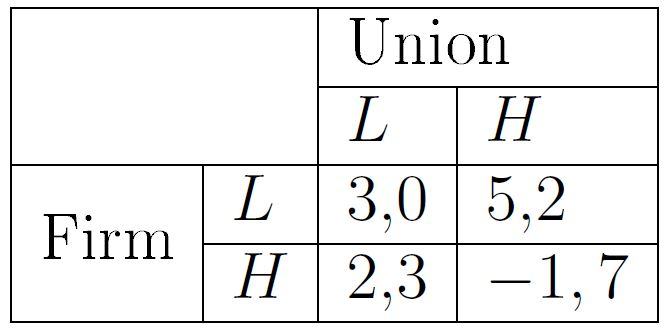
\includegraphics[width=0.5\textwidth]{seventh}
		\end{center}
		
		 Равновесием по Нэшу будет пара стратегий $(L,H)$.
		Всюду далее полагаем $r^f= 4 $ (количество ходов фирмы за одну игру),
		$r^p= 3$ (количество ходов профсоюза). 
\end{frame}


\begin{frame}
\frametitle{Конфликт профсоюз---монополист. Имитация}
	 \begin{gather*}
	 q^f = \left[ 0.9; 0.9; 0.9; 0.9 \right], \\
	 q^p = \left[ 0.1; 0.1; 0.1 \right].
	 \end{gather*}
		\begin{figure}
			\begin{minipage}[b]{0.45\textwidth}
				
				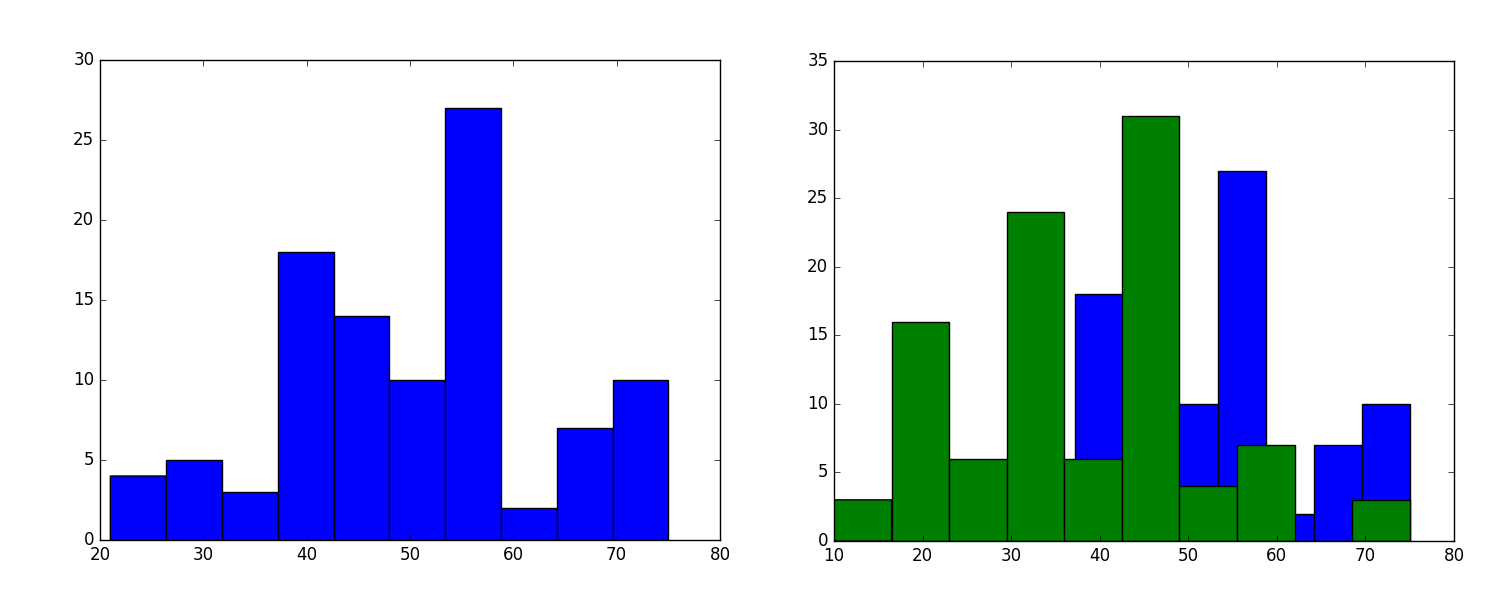
\includegraphics[width=\textwidth]{firm1}
			\end{minipage}
			\begin{minipage}[b]{0.45\textwidth}
				
				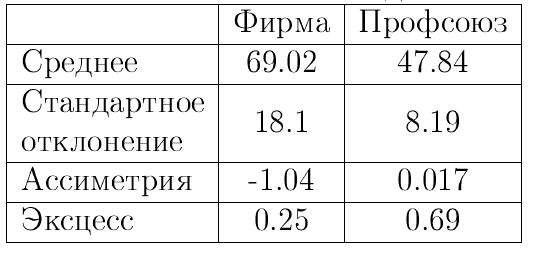
\includegraphics[width=\textwidth]{firmtable1}
			\end{minipage}
			
		\end{figure}
\end{frame}

\begin{frame}
\frametitle{Конфликт профсоюз---монополист. Имитация}
 \begin{gather*}
 q^f = \left[ 0.9; 0.9; 0.9; 0.1 \right], \\
 q^p = \left[ 0.1; 0.1; 0.9 \right].
 \end{gather*}
	\begin{figure}
		\begin{minipage}[b]{0.45\textwidth}
			
			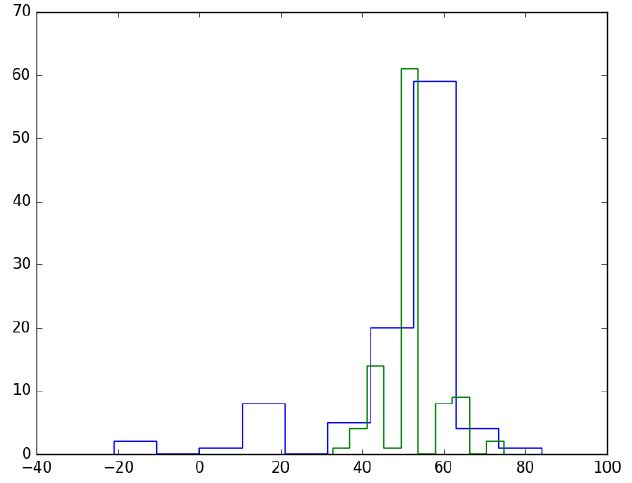
\includegraphics[width=\textwidth]{firm2}
		\end{minipage}
		\begin{minipage}[b]{0.45\textwidth}
			
			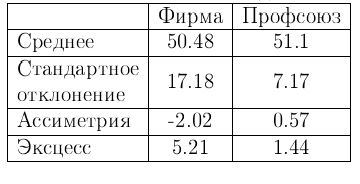
\includegraphics[width=\textwidth]{firmtable2}
		\end{minipage}
		
	\end{figure}
\end{frame}

\begin{frame}
\frametitle{Конфликт профсоюз---монополист. Имитация}
 \begin{gather*}
 q^f = \left[ 0.9; 0.9; 0.1; 0.9 \right], \\
 q^p = \left[ 0.1; 0.9; 0.1 \right].
 \end{gather*}
	\begin{figure}
		\begin{minipage}[b]{0.45\textwidth}
			
			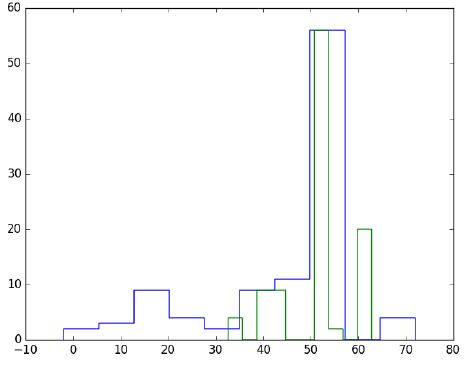
\includegraphics[width=\textwidth]{firm3}
		\end{minipage}
		\begin{minipage}[b]{0.45\textwidth}
			
			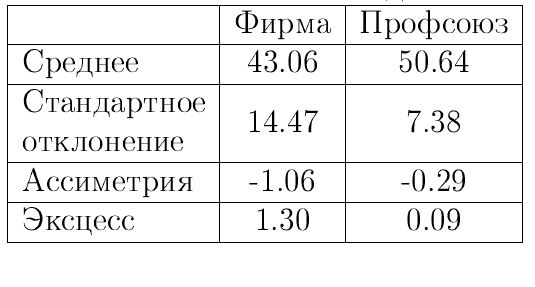
\includegraphics[width=\textwidth]{firmtable3}
		\end{minipage}
		
	\end{figure}
\end{frame}

\begin{frame}
\frametitle{Конфликт профсоюз---монополист. Имитация}
  \begin{gather*}
  q^f = \left[ 0.9; 0.9; 0.1; 0.2 \right], \\
  q^p = \left[ 0.1; 0.9; 0.8 \right].
  \end{gather*}
	\begin{figure}
		\begin{minipage}[b]{0.45\textwidth}
			
			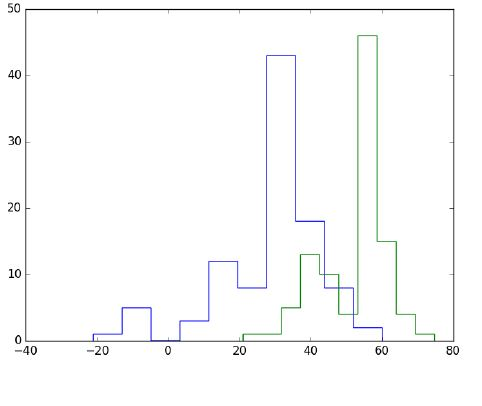
\includegraphics[width=\textwidth]{firm4}
		\end{minipage}
		\begin{minipage}[b]{0.45\textwidth}
			
			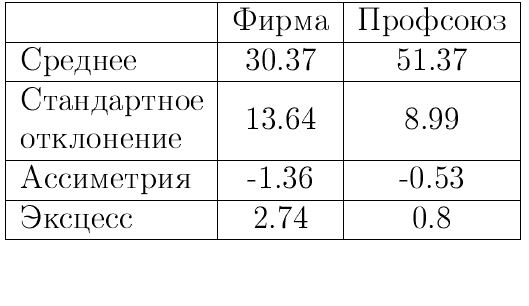
\includegraphics[width=\textwidth]{firmtable4}
		\end{minipage}
		
	\end{figure}
\end{frame}



\begin{frame}
\frametitle{Конфликт профсоюз---монополист. Имитация}
\begin{itemize}
	\item	Фирма, отклоняясь от стратегии низкого найма теряет возможную выгоду, 
		в то время как профсоюз только незначительно улучшает своё положение. 

	\item 	С точки зрения фирмы представляется разумным предложить профсоюзу не требовать 
		высокого уровня зарплат, пообещав компенсировать это индивидуальными бонусами.
\end{itemize}
\end{frame}


\begin{frame}
\frametitle{Выводы}
Выводы\\
\end{frame}

\begin{frame}
\frametitle{Заключение}
Спасибо за внимание!\\
\end{frame}

\end{document}
